\Solution{1: Multi-armed Bandits}
\\

\noindent Code available at: \url{http://tinyurl.com/cs780-assignment-1-p1}
\begin{enumerate}
    \item Created the environment using Gymnasium library. The environment is a 2-armed bernoulli bandit with some stochasticity. The environment characteristics are taken from a config file which specify the $\alpha$ and $\beta$ values. I tested out with different values of $\alpha$ and $\beta$ $[(0,0), (0,1), (1,0), (1,1), (0.5,0.5)]$ and the environment is working as expected. The agent recieves a reward only if it takes an action which takes it correctly in the direction of movement. That is if the the agent moves `left' and lands in state $1$ or moves `right' and lands in state $2$, only then it gets a positive reward. 
    
    \item I created a similar environment with 10-arms just like the above. But in this case the environment is not stochastic. The action and state-transitions are deterministic. The expected reward for each action $q_*(s, a)$ is sampled from a standard normal distribution ($\mathcal{N}(0, 1)$). The agent then receives a reward from a normal distribution with mean $q_*(s, a)$ and variance $1$. The agent has to then learn the optimal action to take in each state, by taking actions and observing the rewards.
    
    \item I created 6 types of bandit agents following different strategies to solve the bandit problem. The agents are:
    \begin{enumerate}
        \item Greedy Agent: This agent always takes the action with the highest estimated value. It does not explore the environment.
        \item Epsilon-Greedy Agent: This agent takes the action with the highest estimated value with probability $1-\epsilon$ and takes a random action with probability $\epsilon$.
        \item Decaying Epsilon-Greedy Agent: This agent is similar to the epsilon-greedy agent, but the value of $\epsilon$ decays ``linearly'' $\epsilon=max(0, \epsilon_0 - decay\_rate * episode)$ or ``exponentially'' $\epsilon=\epsilon_0e^{-decay\_rate*episode}$ with time. 
        \item Softmax Agent: This agent takes actions with probability proportional to the exponential of the estimated value of the action. The agent explores the environment by taking actions by choosing from the below distribution
        \begin{equation}
            \pi(a|s) = \frac{e^{Q(s,a)/\tau}}{\sum_{b}e^{Q(s,b)/\tau}}
        \end{equation}
        \item UCB Agent: This agent takes actions by choosing the action with the highest upper confidence bound. The upper confidence bound is calculated as $Q(s,a) + c\sqrt{\frac{\ln t}{N(s,a)}}$ where $c$ is a constant and $N(s,a)$ is the number of times the action $a$ has been taken in state $s$. The action is taken by taking the argmax of the upper confidence bound. 
    \end{enumerate}
    
    \item Created 50 different bandit problems for 2-armed Bernoulli Bandit with $\alpha$ and $\beta$ values chosen from uniform distribution $\mathcal{U}(0, 1)$. The agents were then tested on these bandit problems. The agents were tested for 1000 episodes and the average reward, average regret and optimal action percentage was calculated. The results are shown in the plots below (Figure \ref{fig:bernoulli_reward}, \ref{fig:bernoulli_regret}, \ref{fig:bernoulli_optimal_action}). 
    
    \item Created 50 different bandit problems for 10-armed Gaussain Bandit with $q_*(s, a)$ values chosen from standard normal distribution $\mathcal{N}(0, 1)$ and then the agent receives a reward from $\mathcal{N}(q_*(s, a), 1) \forall a \in A$. The agents were then tested on these bandit problems for 1000 episodes and the average reward, average regret and optimal action percentage was calculated. The results are shown in the plots below (Figure \ref{fig:gaussian_reward}, \ref{fig:gaussian_regret}, \ref{fig:gaussian_optimal_action}).
    
    \begin{figure}[h]
        \centering
        \begin{subfigure}[b]{0.3\textwidth}
            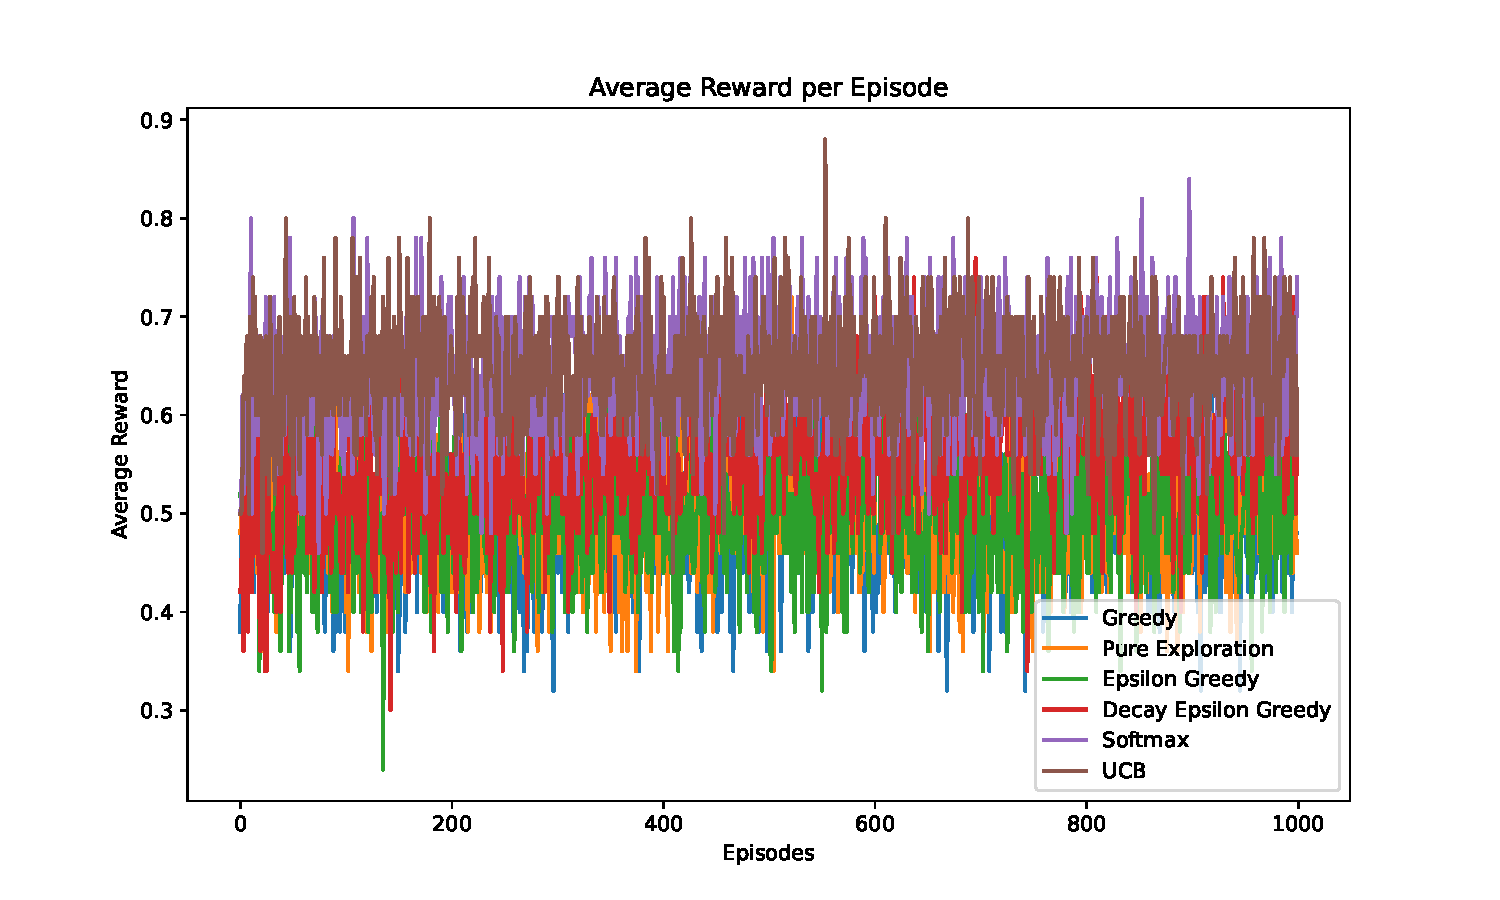
\includegraphics[width=\textwidth]{images/mab/bernoulli_average_reward_per_episode.pdf}
            \caption{Average reward}
            \label{fig:bernoulli_reward}
        \end{subfigure}

        \begin{subfigure}[b]{0.3\textwidth}
            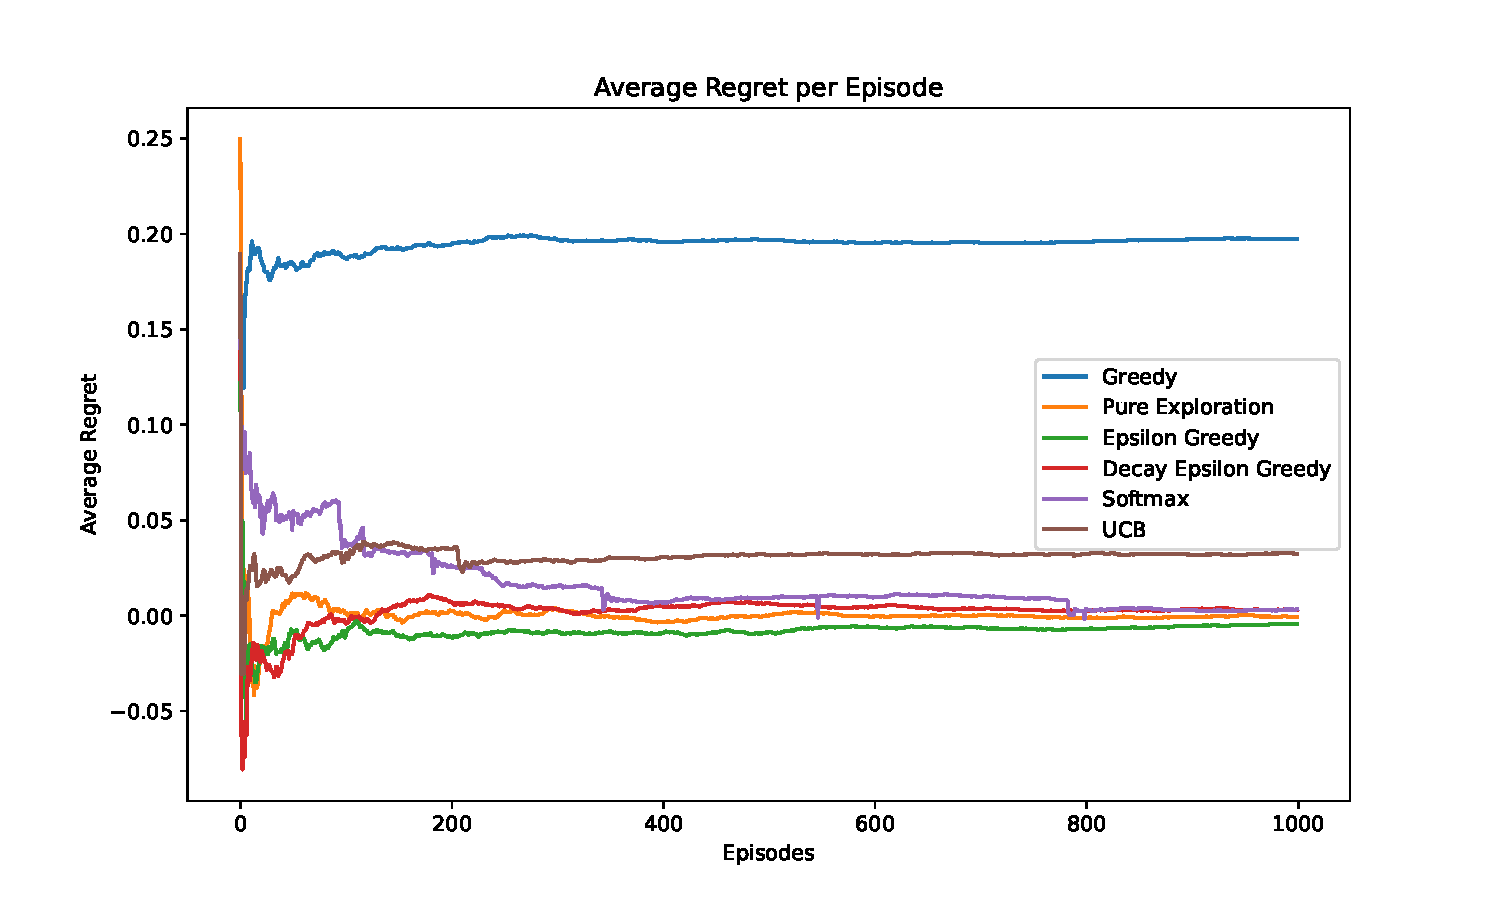
\includegraphics[width=\textwidth]{images/mab/bernoulli_average_regret_per_episode.pdf}
            \caption{Average regret}
            \label{fig:bernoulli_regret}
        \end{subfigure}

        \begin{subfigure}[b]{0.3\textwidth}
            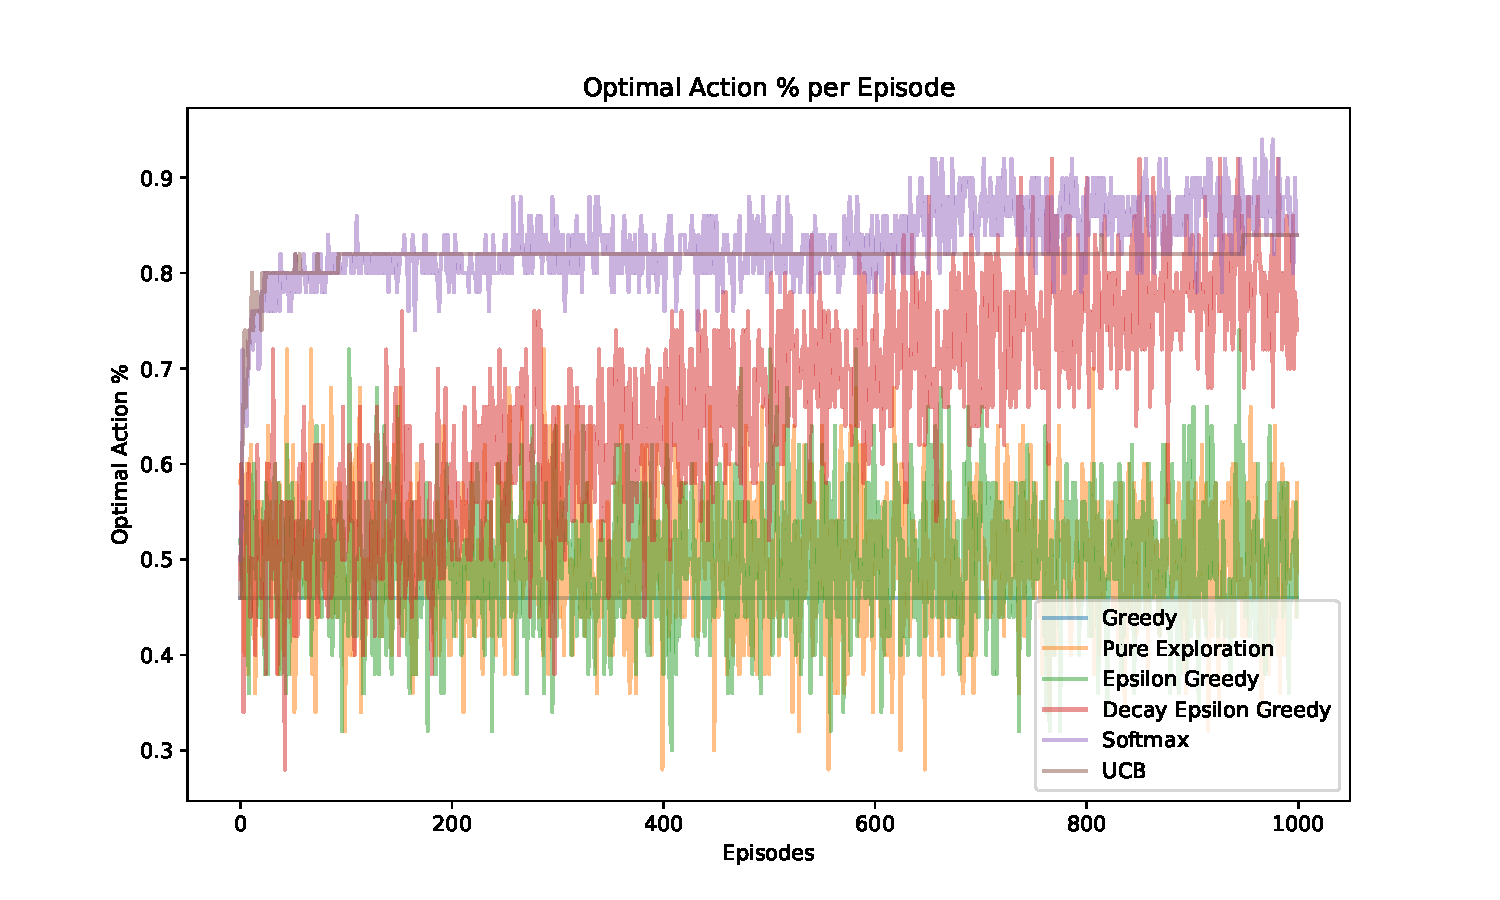
\includegraphics[width=\textwidth]{images/mab/bernoulli_optimal_actions_percentage_per_episode.pdf}
            \caption{Optimal Action \%}
            \label{fig:bernoulli_optimal_action}
        \end{subfigure}
        \caption{Results of 2-armed Bernoulli Bandit}

    \end{figure}

    \item Created a plot of the average regret of the agents for the 2-armed Bernoulli Bandit. Figure \ref{fig:bernoulli_regret} shows the average regret of the agents for the 2-armed Bernoulli Bandit. From the plot we can see that Greedy agent has the highest regret and it is continuously increasing. The epsilon-greedy and pure exploration agents have similar regret values. The regret of epsilon-decay rises as it is exploring but flattens out once it is confident about its environment. While the UBC and Softmax agents do not have much regret.
    

    \item Created a plot of the average regret of the agents for the 10-armed Gaussian Bandit. Figure \ref{fig:gaussian_regret} shows the average regret of the agents for the 10-armed Gaussian Bandit. From the plot we can see that Pure exploration leads to random reward retrivals making the agent gather more regret. The epsilon-greedy, epsilon-decay and UCB agents have similar regret values. While the greedy and softmax agents are very similar in regret values. We also notice that the regret does not sigificantly flatten out for any agent. Thus, we may need to run more steps to see the regret flatten out.
    \begin{figure}[h]
        \centering
        \begin{subfigure}[b]{0.3\textwidth}
            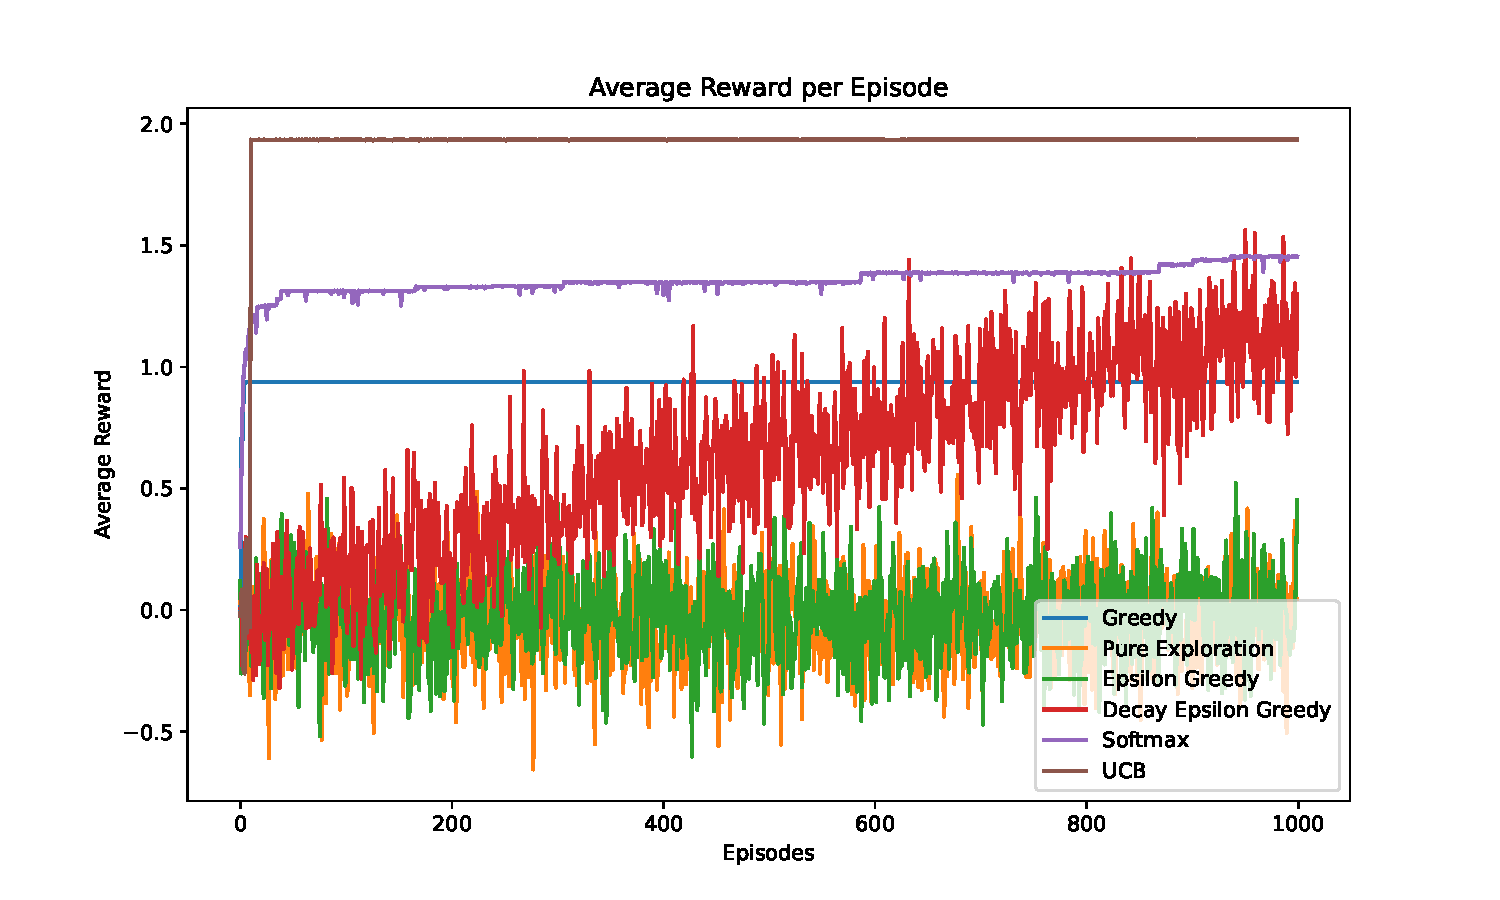
\includegraphics[width=\textwidth]{images/mab/10_arm_gaussian_average_reward_per_episode.pdf}
            \caption{Average reward}
            \label{fig:gaussian_reward}
        \end{subfigure}
        \begin{subfigure}[b]{0.3\textwidth}
            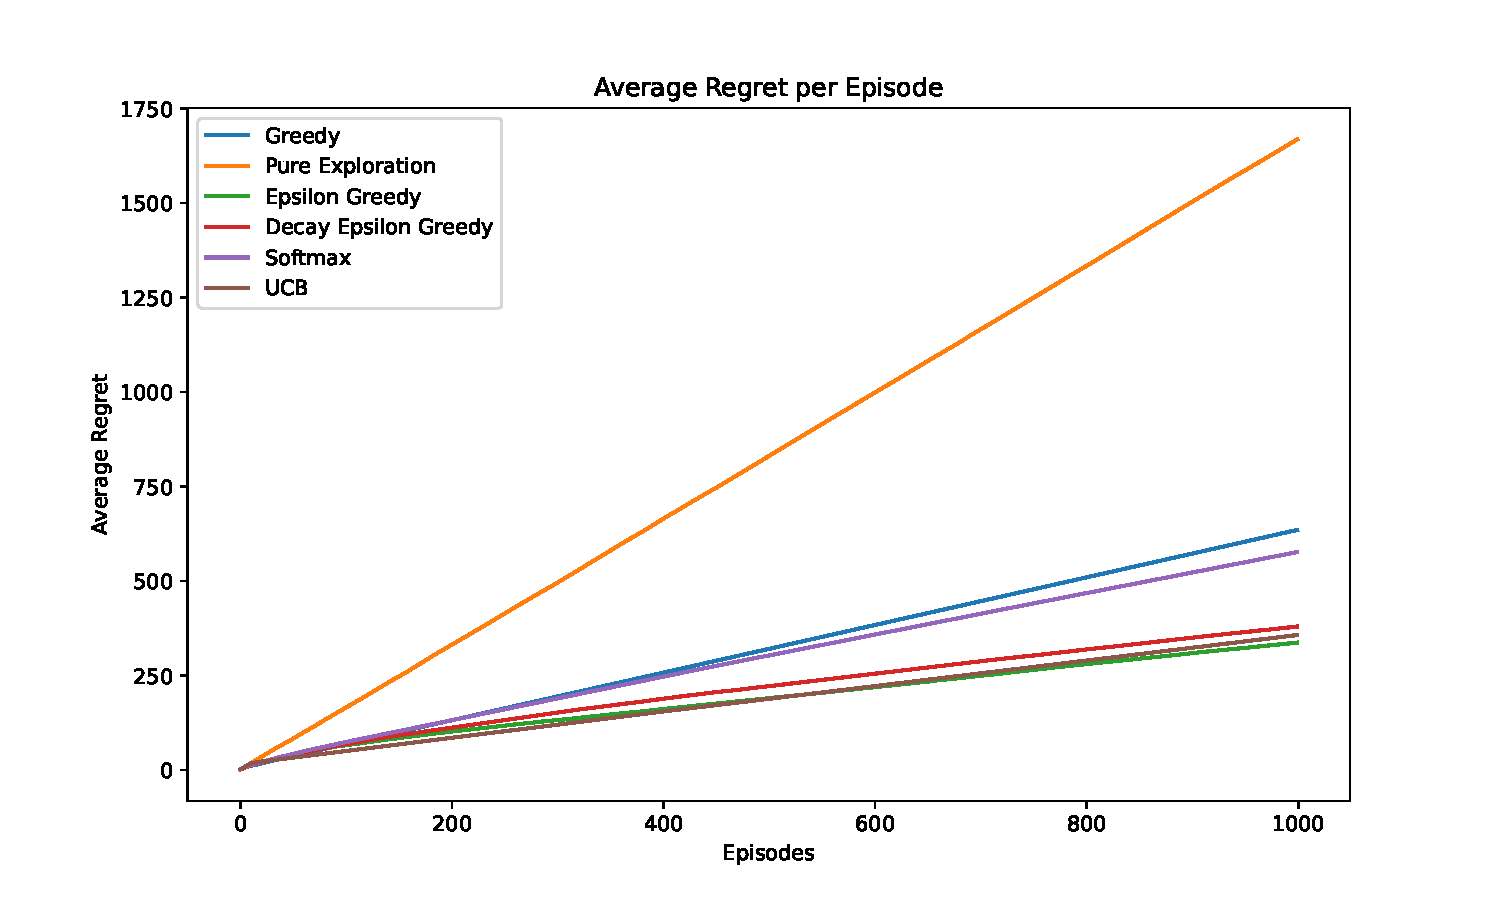
\includegraphics[width=\textwidth]{images/mab/10_arm_gaussian_average_regret_per_episode.pdf}
            \caption{Average regret}
            \label{fig:gaussian_regret}
        \end{subfigure}
        \begin{subfigure}[b]{0.3\textwidth}
            \centering
            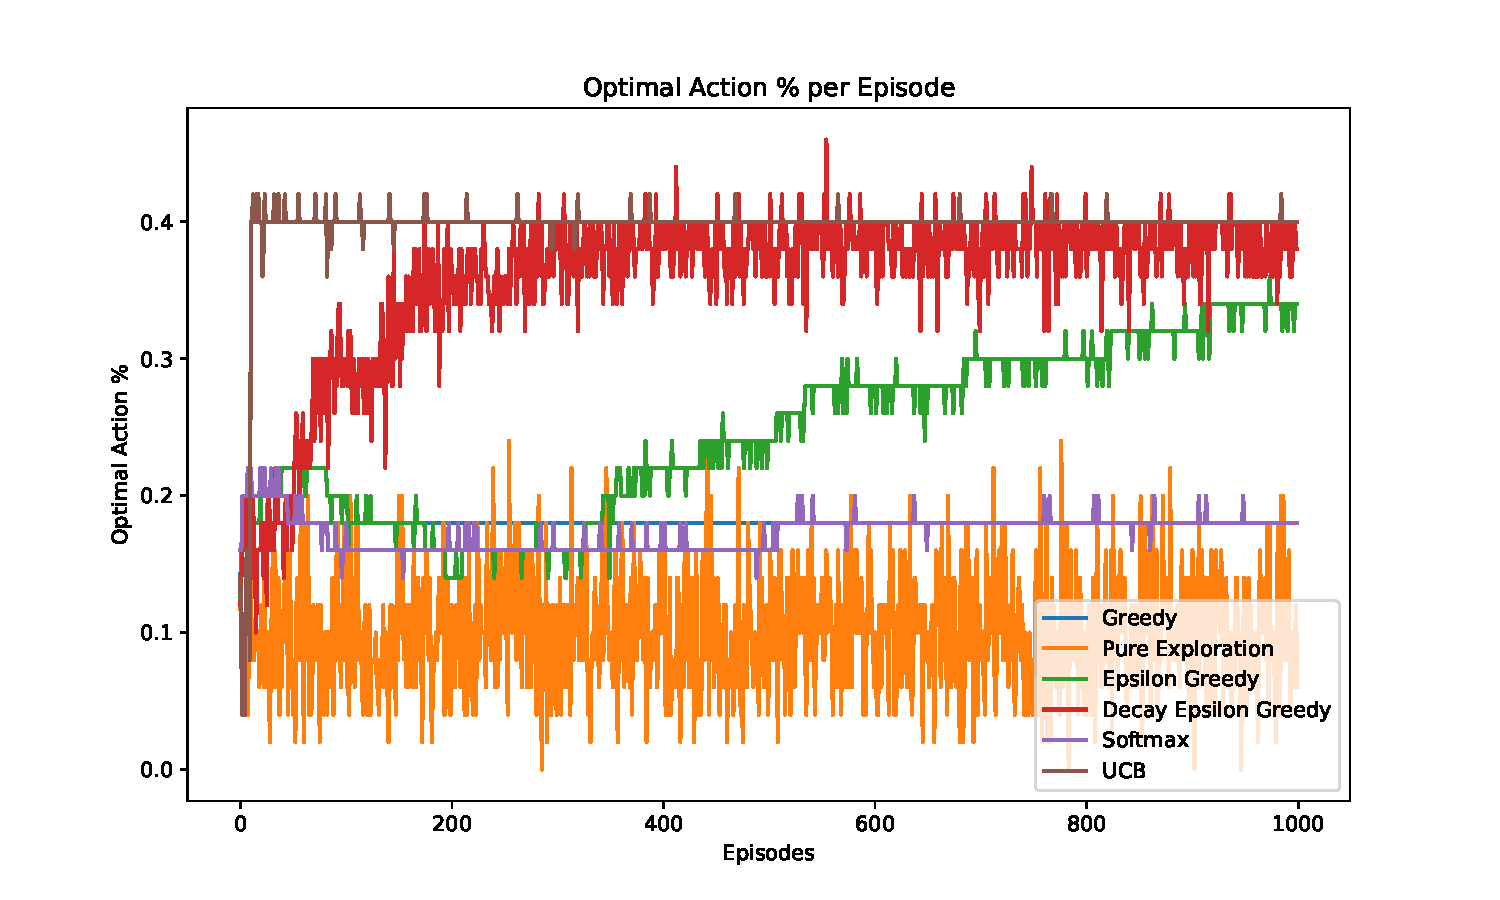
\includegraphics[width=\textwidth]{images/mab/10_arm_gaussian_optimal_actions_percentage_per_episode.pdf}
            \caption{Optimal Action \%}
            \label{fig:gaussian_optimal_action}
        \end{subfigure}
        \caption{Results of 10-armed Gaussian Bandit}
        
    \end{figure}

    \item This is the same as question 4. 
    
    \item Plotting the optimal action percentage of each agent for the 2-armed Bernoulli Bandit. Running 50 experiments did not reduce the variance by a noticeable margin, making the plots look very noisy. The results are shown in Figure \ref{fig:bernoulli_optimal_action}. From the plot we can see that the greedy agent has the lowest optimal action percentage. The epsilon-greedy and pure exploration agents have similar optimal action percentage, which means I have to change the eplison value even more. The UCB and Softmax agents have the highest optimal action percentage. While the epsilon-decay agent shows potential as its optimal action percentage increases with time. Running more expisodes could've proven the epsilon-decay agent to be the best.

    \item Plotting the optimal action percentage of each agent for the 10-armed Gaussian Bandit. The plots here are not as noisy as the 2-armed Bernoulli Bandit. The results are shown in Figure \ref{fig:gaussian_optimal_action}. From the plot we can see that the Pure exploration has the lowest optimal action percentage, which is inline with the regret plot of Pure exploration. This is followed by greedy and softmax agents. The optimal-action percentage plot shows that epsilon-greedy and epsilon-decay agents have the best action selection strategy and beat UCB agent by a noticeable margin, which is not evident from the regret plots.
    

\end{enumerate}